% PLEASE USE THIS FILE AS A TEMPLATE
% Check file iosart2x.tex for more examples

% add. options: [seceqn,secthm,crcready] FC:original:[sw]
\documentclass[crcready]{iosart2x}

%\usepackage{dcolumn}

\usepackage{comment} %% utility package: allows multiline comments
\usepackage{xspace} %% utility package: allows definition of no-argument commands that do not absorb trailing saces
\usepackage{ifthen} %% utility package: allows for conditionals
\usepackage{xcolor} %% utility package: colors for temporary comments

%%%%%%%%%%%%%%%%%%%%%%%%%%%%%%%%%%%%%%%%%%%%%%%%%%%%%%%%%%%%%%%%%%%%%%%%%%%%%%%%%%%%%%%5
%%%%%%%%%%% Put your definitions here
%%%%% FORMULAS
% COUNTERS
% newcommand for list ox formula environment
\newcommand{\bflist}{\begin{list}{}{\setlength{\topsep}{2mm}\setlength{\partopsep}{0mm}\setlength{\parsep}{0mm}\setlength{\leftmargin}{9mm}\setlength{\labelwidth}{8mm}}}
    \newcommand{\eflist}{\end{list}}
    
    % newcommand for labels of axioms, definitions and formulae
    \newcommand{\AxLabel}{\textrm{a}}
    \newcommand{\DefLabel}{\textrm{d}}
    \newcommand{\ExLabel}{\textrm{ex}}
    \newcommand{\FmLabel}{\textrm{f}}
    \newcommand{\ThrLabel}{\textrm{t}}
    
    % counter and newcommand for numbering formulas
    \newcounter{cntax}
    \newcommand{\myax}[1]{\refstepcounter{cntax}\begin{small}{\bf \AxLabel\thecntax\label{ax:#1}}\end{small}}
    \newcounter{cntdef}
    \newcommand{\mydf}[1]{\refstepcounter{cntdef}\begin{small}{\bf \DefLabel\thecntdef\label{def:#1}}\end{small}}
    \newcounter{cntfm}
    \newcommand{\myex}[1]{\refstepcounter{cntex}\begin{small}{\bf \ExLabel\thecntex\label{ex:#1}}\end{small}}
    \newcounter{cntex}
    \newcommand{\myfm}[1]{\refstepcounter{cntfm}\begin{small}{\bf \FmLabel\thecntfm\label{for:#1}}\end{small}}
    \newcounter{cntthr}
    \newcommand{\mythr}[1]{\refstepcounter{cntthr}\begin{small}{\bf \ThrLabel\thecntthr\label{th:#1}}\end{small}}
    
    \newcommand{\mytext}[1]{``#1''}
    
    \newcommand{\refax}[1]{({\AxLabel}\ref{#1})}
    \newcommand{\refdf}[1]{({\DefLabel}\ref{#1})}
    \newcommand{\refex}[1]{({\ExLabel}\ref{#1})}
    \newcommand{\reffm}[1]{({\FmLabel}\ref{#1})}
    \newcommand{\refth}[1]{({\ThrLabel}\ref{#1})}

%%%%% Predicates styling
%% general style -- purtroppo non funzionano tutti siccome LaTeX fa le storie per le espansioni delle macro, credo
%                 - però almeno texttt, textnormal, textbf e textit funzionano; textsc non funziona
\newcommand{\generalStyle}[1]{\texttt{#1}}
%% binary predicate style
\newcommand{\biRel}[3]{\generalStyle{#1}(#2,#3)}
%% monadic predicate style
\newcommand{\uniRel}[2]{\generalStyle{#1}(#2)}
%% monadic predicate (parameterized) style
\newcommand{\uniRelPar}[3]{\generalStyle{#1}_{\generalStyle{#3}}(#2)}
%% binary predicate (parameterized) style
\newcommand{\biRelPar}[4]{\generalStyle{#1}_{\generalStyle{#4}}(#2,#3)}
%% ternary predicate style
\newcommand{\triRel}[4]{\generalStyle{#1}(#2,#3,#4)}
%% constant style
\newcommand{\cst}[1]{\ensuremath{\mathtt{#1}}}


%%%%%%% Logic symbols
%% biconditional
\newcommand{\myiff}{\Longleftrightarrow}
%% necessary condition
\newcommand{\myif}{\Longleftarrow \hspace{0.9mm}}
%% sufficient condition
\newcommand{\myfi}{\hspace{0.9mm} \Longrightarrow}

%%%%%%% DOLCE
%% DOLCE style -- Small Caps, ie textsc, non funziona per qualche ragione
\newcommand{\DOLCE}{\textsc{DOLCE}\xspace} %% TODO far si che le macro applichino lo stile :(, perche' textsc non funziona?
\newcommand{\YAMATO}{\textsc{YAMATO}\xspace}
\newcommand{\BFO}{\textsc{BFO}\xspace} 
\newcommand{\GFO}{\textsc{GFO}\xspace} 
\newcommand{\OWL}{\textnormal{OWL}\xspace} 

%% DOLCE various predicates
\newcommand{\DOLCEQuality}[1]{\uniRel{Q}{#1}}
\newcommand{\DOLCEQualityDirect}[2]{\biRel{qt}{#1}{#2}}
\newcommand{\DOLCEQualeDirect}[2]{\biRel{{ql}}{#1}{#2}}
\newcommand{\DOLCEPart}[2]{\biRel{{P}}{#1}{#2}}
\newcommand{\DOLCEEvent}[1]{\uniRel{{E}}{#1}}
\newcommand{\DOLCEDescription}[1]{\uniRel{{D}}{#1}}
\newcommand{\DOLCEAgent}[1]{\uniRel{{ASO}}{#1}}
\newcommand{\DOLCECLby}[3][]{\biRelPar{{CL}}{#2}{#3}{#1}}
\newcommand{\Role}[1]{\uniRel{{Role}}{#1}}
\newcommand{\DOLCEState}[1]{\uniRel{{ST}}{#1}}
\newcommand{\DOLCEProcess}[1]{\uniRel{PRO}{#1}}
\newcommand{\DOLCEPerdurant}[1]{\uniRel{{PER}}{#1}}
\newcommand{\DOLCEPhysObj}[1]{\uniRel{{POB}}{#1}}
\newcommand{\DOLCESum}[3]{\triRel{Sum}{#1}{#2}{#3}}
%%%% Additional predicates
\newcommand{\TechArt}[1]{\uniRel{TechArt}{#1}}
\newcommand{\Component}[1]{\uniRel{Component}{#1}}
\newcommand{\Capability}[1]{\uniRel{Capability}{#1}}
\newcommand{\PumpingCapability}[1]{\uniRel{PumpingCapability}{#1}}
\newcommand{\PumpingProcess}[1]{\uniRel{PumpingProcess}{#1}}
\newcommand{\BehaviourAbstract}[1]{\uniRel{AbstBeh}{#1}}
\newcommand{\BehaviourConcrete}[1]{\uniRel{Behaviour}{#1}}
\newcommand{\Capacity}[1]{\uniRel{Capacity}{#1}}
\newcommand{\founded}[2]{\biRel{\foundedTerm{passive}}{#1}{#2}}
\newcommand{\partTA}[2]{\biRelPar{P}{#1}{#2}{TA}}
\newcommand{\participateAsDoer}[2]{\biRel{participateAsDoer}{#1}{#2}}
\newcommand{\describedBy}[2]{\biRelPar{described-by}{#1}{#2}{Cap}}
\newcommand{\realizedIn}[2]{\biRelPar{realized-in}{#1}{#2}{Beh}}
\newcommand{\behSum}[3]{\triRel{Sum}{#1}{#2}{#3}}
\newcommand{\DOLCEQualeTer}[3]{\triRel{ql}{#1}{#2}{#3}}

%% Fnctional Basis Thingies
\newcommand{\Flow}[1]{\uniRel{Flow}{#1}}
\newcommand{\flowOf}[2]{\biRel{flowOf}{#1}{#2}}
\newcommand{\Energy}[1]{\uniRel{Energy}{#1}}
\newcommand{\Material}[1]{\uniRel{Material}{#1}}
\newcommand{\Signal}[1]{\uniRel{Signal}{#1}}
\newcommand{\inp}[2]{\biRel{inp}{#1}{#2}}
\newcommand{\out}[2]{\biRel{out}{#1}{#2}}
\newcommand{\ABSum}[3]{\triRel{ASum}{#1}{#2}{#3}}

%%%% First time keyword - usare quando una parola chiave è menzionata per la prima volta
\newcommand{\firstTimeKeyWord}[1]{\textit{#1}}

%%%% Terminology - termini introdotti dall'articolo, potenzialmente questionabili, da modificare facilmente
%%%%%% Terminologia

%% individual quality founds capability
\newcommand{\foundedTerm}[1]{%
  \ifthenelse{\equal{#1}{passive}}{founded}{%
    \ifthenelse{\equal{#1}{verb}}{found}{%
      \ifthenelse{\equal{#1}{gerund}}{founding}{%
        ERROR!%
      }%
    }%
  }%
}  
%%%%%%%%%%%%%%%%%%%%%%%%%%%%%%%%%%%%%%%% miscellanea
%%%%%% The following 4 lines are from https://tex.stackexchange.com/questions/287081/how-to-prevent-a-linebreak-before-align-equation-environment-in-itemize/287091#287091
\newcommand{\myalignspaceskip}{
 \abovedisplayskip=-\baselineskip
 \belowdisplayskip=0pt
 \abovedisplayshortskip=-\baselineskip
 \belowdisplayshortskip=0pt}
%%%%%% Commenti
\newcommand{\TODO}[1]{{\color{red} #1}}
%%%%%%%%%%%%%%%%%%%%%%%%%%%%%%%%%%%%%%%%
%%%%%%%%%%% End of definitions
%%%%%%%%%%%%%%%%%%%%%%%%%%%%%%%%%%%%%%%%%%%%%%%%%%%%%%%%%%%%%%%%%%%%%%%%%%%%%%%%%%%%

\pubyear{0000}
\volume{0}
\firstpage{1}
\lastpage{1}

\begin{document}

\begin{frontmatter}

%\pretitle{}
\title{About functions, behaviours, and capabilities in formal ontology and engineering}
\runtitle{Running head title}
%\subtitle{}

% For one author:
%\author{\inits{N.}\fnms{Name1} \snm{Surname1}\ead[label=e1]{first@somewhere.com}}
%\address{Department first, \orgname{University or Company name},
%Abbreviate US states, \cny{Country}\printead[presep={\\}]{e1}}

% Two or more authors:
\begin{aug}
\author[A]{\inits{N.}\fnms{Name1} \snm{Surname1}\ead[label=e1]{first@somewhere.com}%
\thanks{Corresponding author. \printead{e1}.}}
\author[B]{\inits{N.N.}\fnms{Name2 Name2} \snm{Surname2}\ead[label=e2]{second@somewhere.com}}
\author[B]{\inits{N.-N.}\fnms{Name3-Name3} \snm{Surname3}\ead[label=e3]{third@somewhere.com}}
\address[A]{Department first, \orgname{University or Company name},
Abbreviate US states, \cny{Country}\printead[presep={\\}]{e1}}
\address[B]{Department first, \orgname{University or Company name},
Abbreviate US states, \cny{Country}\printead[presep={\\}]{e2,e3}}
\end{aug}

%\begin{review}{editor}
%\reviewer{\fnms{First} \snm{Editor}\address{\orgname{University or Company name}, \cny{Country}}}
%\reviewer{\fnms{Second} \snm{Editor}\address{\orgname{First University or Company name}, \cny{Country}
%    and \orgname{Second University or Company name}, \cny{Country}}}
%\end{review}
%\begin{review}{solicited}
%\reviewer{\fnms{First} \snm{Solicited reviewer}\address{\orgname{University or Company name}, \cny{Country}}}
%\reviewer{\snm{anonymous reviewer}}
%\end{review}
%\begin{review}{open}
%\reviewer{\fnms{First} \snm{Open Reviewer}\address{\orgname{University or Company name}, \cny{Country}}}
%\end{review}

\begin{abstract}
    %% NOTA (estratti dal testo della call):
    %... industrial environments where machines are designed to smoothly interact between themselves and with humans via knowledge models. 
    %At the same time, however, 
    %practitioners and stakeholders lack methodologies and guidelines to reliably develop, use or integrate (existing) ontologies ...
    %% (elenco alcuni temi)
    %-...
    %-Ontologies for knowledge representation and reasoning about topics relevant for industrial engineering (e.g., products, processes, manufacturing resources, requirements and capabilities, etc.).
    %-Ontology-based patterns for industrial engineering knowledge representation.
    %-ethodologies, methods, and techniques targeted to industrial contexts supporting the development, modularization, extension, and evolution of ontologies.
    %-Literature review of existing ontologies for industrial engineering, including structured comparisons.
    %-Experiences with the use of top-level ontologies (e.g. BFO, DOLCE, ISO 15926, among others) in industrial engineering.
    %-Experiences with research and application initiatives such as OntoCommons, the Industry Ontologies Foundry (IOF), and the UK National Digital Twins.

    %% NOTA (estratti dal file iosart2x.pdf)
    %...
    %– The use of first persons (i.e., “I”, “we”, “their”, possessives, etc.) should be avoided, and can preferably be
    %expressed by the passive voice or other ways. This also applies to the Abstract.
    %– A research paper should be structured in terms of four parts, each of which may comprise of multiple sections:
    %   * Part One is problem description/definition, and a literature review upon the state of the art.
    %   * Part Two is methodological formulation and/or theoretical development (fundamentals, principle and/or ap-
    %     proach, etc.).
    %   * Part Three is prototyping, case study or experiment.
    %   * Part Four is critical evaluation against related works, and the conclusion.
    %In any article it is unnecessary to have an arrangement statement at the beginning (or end) of every (sub-) section.
    %Rather, a single overall arrangement statement about the whole paper can be made at the end of the Introduction
    %section. ...

    In both applied ontology and engineering, a rich portion of the literature has researched ways to represent the functionality of engineering systems. 
    Such a topic is of fundamental importance, since it is through teleological causal reasoning, which gives birth to functions, that domain experts build mental 
    models of machines and the like. 
    Furthermore, functionality is important throughout the whole lifecycle of any product, being used from the design phase to any eventual
    diagnosis activity. 

    A vast amount of work has already been done, even so the literature has not settled on a unique and well-defined methodology. 
    This work develops preliminary steps towards an ontological description of functions and related concepts, such as behaviour and capability.
    This is accomplished through a conceptual analysis of the fundamental notions related to functionality, carried out using the top level ontology \DOLCE as a framework for reference. 
    A formal description is given in \TODO{first order logic/???} \OWL, and some examples are worked through.
    
\end{abstract}

\begin{keyword} 
    %% NOTA
    % ... Please include 3-7 keywords below the abstract of your manuscript. ... 
\kwd{Ontology}
\kwd{Function}
\kwd{Behaviour}
\kwd{Capability}
\end{keyword}

\end{frontmatter}

%%%%%%%%%%%%%%%%%%%%%%%%%%%%%%%%%% ELENCO Di TODOS
%% TODO sostituire 'I', 'us', 'we', 'our', etc. con costrutti alternativi, come da linee guida stilistiche
%% TODO aggiustare l'uso indiscriminato del genitico sassone
%%%%%%%%%%%%%%%%%%%%%%%%%%%%%%%%%% FINE TODOS

%%%%%%%%%%% The article body starts:


\section{Introduction}\label{sec:intro}
Functionality is a concept that has interested engineers as well as philosophers and applied ontologists.
In particular, due to strong practical interests, a vast literature within engineering has been developed. Fundamental works are, for example, 
 \cite{de_kleer_how_1984, kleer_qualitative_1984}, which outlines foundational principles such as the locality of functions (functions of a component should refer only to neighboring entities)
 and the `no function in structure' principle (structural models should not contain teleological information); and \cite{pahl_engineering_2007}, which describes functions as black-box transformations applied to input flows, divides functions based on the property of the flow 
 acted upon (e.g., quantity, type, position, etc.), and discusses function decomposition (that is, how to achieve a given function through a structure of adequate subfunctions).

 The definition of functions as (selected) actions on flows is the most common type encountered in the engineering literature, for example \cite{chandrasekaranFunctionalRepresentationDesign1993} speaks of  ``intended input-output relations'', and different vocabularies were proposed in order to 
 standardize function terminology. Many vocabularies were proposed, from the simple four terms (toMake, toMantain, toPrevent, and toControl) of \cite{keuneke_device_1991}, 
 to bigger vocabularies built using complex algorithms \cite{kitamuraFunctionalConceptOntology2002a}. 
 A common example is the Functional Basis \cite{hirtz_functional_2002, stone_development_2000}, that gives terms for 
 actions and flows on a three-levels taxonomy described in natural language.

 The literature about the use of such vocabularies has not settled yet and, currently, different lines of research are being pursued, such as behavioural simulation of a system from the functional model \cite{kurtogluGraphBasedFaultIdentification2008} or 
 formal description and automatic construction of the 
 functional model itself \cite{gill_logic_2021,kurtoglu_automating_2010}.

 %These vocabularies equate functions to transformations of objects, thus using verbs or verbs-objects[nouns] pair as terms. 

It is generally recognized that functionality depends on the intention of an agent, a typical example being the designer's one \cite{kitamuraOntologyBasedFunctionalKnowledgeModeling2004}, also called `design rationale' \cite{chandrasekaranFunctionalRepresentationDesign1993}. 
Thus, functions are not objective, at least not completely. Then, it is natural to wonder what in a function is fully objective. Behaviour, intended as what a device does, as determined by physical laws, is usually the answer.    

%Also for the term behaviour we have no universally shared definition, but such a concept is usually countraposed to `function'. Some authors say that behaviour is what  
Even for the term behaviour we have ambiguous use and no universally shared definition. Some authors classified the multiple uses of `behavior' in engineering literature: 
the work \cite{kitamuraOntologyBasedFunctionalKnowledgeModeling2004} determines four types of devices behaviour (excluding static behaviours such as supporting), depending on whether the device changes another device, its own state, or one of its operands (that either stays in the same position or travels between input and output ports).
Instead, in \cite{chandrasekaranFunctionDeviceRepresentation2000} behaviours are divided mainly depending on their time duration (instant, interval, or unspecified).

%Behaviour themselves are typically recognized as 

\TODO{vedere se inserire qui discorso differenza tra behaviour astratti e concreti}

The link between function and behaviour generally refers to the duality between objectivity and intentionality: some authors state that behaviour is what a device does, whilst function is what a device is for \cite{kleer_qualitative_1984}, 
others focus on describing behaviour as a sequence of state changes and functions as abstractions of behaviours with a goal in mind \cite{umedaFunctionBehaviourStructure1990}. In \cite{sasajimaFBRLFunctionBehavior1995, sasajimaInvestigationDomainOntology1994}, 
it is stated that function is made from behaviour plus additional teleological information called ``functional topping'', which amounts to the selection of (some aspects of) a behaviour, in a way precise enough to distinguish the cases where a device with one behaviour 
has different functions depending on the context. In \cite{chandrasekaranFunctionDeviceRepresentation2000} functions are the sum of intentions and sets of behavioural constraints, defined, essentially, as causal relations between devices'states.

\TODO{differenza tra implementation way e resto?}

In any case, to date numerous systems have been developed in order to deal with functional and behavioural representation of an engineering systems 
(e.g., FBS \cite{umedaFunctionBehaviourStructure1990}, FBRL \cite{sasajimaFBRLFunctionBehavior1995}, FR \cite{sembugamoorthy1986functional}, 
SBF \cite{goelUseDesignPatterns2004}, FBS \cite{qianFunctionBehaviorStructure1996}, etc.\footnote{To briefly explain some distinctions \TODO{distinguere i 2 FBS}.}). 

Most of such systems come from the engineering community and tend not to be interoperable or grounded in ontological theories, even though that could be quite beneficial, especially 
because of the vast number of such systems and the high attention kept on terminological matters. 
Moreover, they often do not make use of formal languages such as first order logic or \OWL, instead preferring informal descriptions in natural language or pseudocode (actually, 
\cite{kitamuraOntologicalModelDevice2006} and \cite{yangFunctionSemanticRepresentation2010} %
%, and \cite{senProtocolFormaliseFunction2011} 
showcase an implementation of a renewed and industrially deployed version of FBRL, called SOFAST, using the ontology editor Hozo, and 
an \OWL and SWRL formalisation of the Functional Basis %
% and a pseudocode and logical formalisation of the Functional Basis 
respectively).
In addition, some topics such as the link between function and malfunction, the difference between function and behaviour, or the methodology with which to carry out the decomposition of a function have been tackled many times but still remain murky.

Despite the clear utility of an ontological analysis of these topics, the attempts carried until now don't give a full picture. 
A few research works have formalized part of the FR system \cite{borgoFormalOntologicalPerspective2009}, started a formalisation of the Functional Basis 
vocabulary (and the conceptualisation it is based on) with the upper ontology \DOLCE \cite{borgoOntologicalRepresentationFunctional2009, borgoFormalizationFunctionsOperations2011}, compared the Functional Basis either with the FR system \cite{garbaczTwoOntologydrivenFormalisations2011} or with both FR and FBRL \cite{kitamuraDeepSemanticMapping2008}. 
Additionally, applied ontology has influenced engineering literature, as shown by the description of functions as roles played by behaviours \cite{mizoguchiUnifiedDefinitionFunction2012, kitamuraOntologicalModelDevice2006, chandrasekaranFunctionDeviceRepresentation2000}, or the classification of behaviours  as occurrents \cite{kitamuraOntologicalModelDevice2006}.

Still, no shared reference ontology of functions exists, and top level ontologies do not explore theories of functions. 
For example, \DOLCE makes no mention of function within its specification \cite{masoloWonderWebDeliverableD182003}, but, additional research work was later developed, in which 
functions are considered as particular types of events, called achievements \cite{borgoCapabilitiesCapacitiesFunctionalities2021}. 

The last version of \YAMATO classifies functions as roles and behaviours as processes caused by an unintentional actor, 
but delegates the description of a functional ontology to a series of additional papers \cite{kitamuraOntologicalModelDevice2006, kitamuraCharacterizingFunctionsBased2013, mizoguchiFunctionalOntologyArtifacts2009}. 

\BFO defines functions as dispositions\footnote{Note that in \BFO functions are dispositions, not roles, while in \YAMATO the opposite holds. See \cite{mizoguchiFunctionalOntologyArtifacts2009} and\cite{spearFunctionsBasicFormal2016} for a comparison.} 
but, other than that, does not commit to an axiomatisation. 
Instead, it clarifies that functions are dispositions that exist in virtue of their bearer's physical make-up, 
and such that the physical make-up came into being
through intentional design (in the case of engineering). 
\GFO too says that functions can be realized by other entities, but makes no mention of dispositions and, instead, calls functions intentional entities \cite{herreGeneralFormalOntology2006}.
The last development of ISO 15926 \cite{kluwerISO159261420202020} adopts \BFO view of functions as dispositions realized in particular processes.

 Then, it is clear that even within the ontology community the meaning of function is ambiguous. Moreover, it is generally not considered 
 a top level concept, and thus it is marginally considered in top level ontologies. Unfortunately, to the knowledge of this author \TODO{to check}, the ontology community 
 has not produced a middle or domain level ontology dealing with functions (the taxonomy of one such an ontology, which is still being developed, was showcased in \cite{borgoCapabilitiesCapacitiesFunctionalities2021} and \cite{borgoKnowledgebasedAdaptiveAgents2019}).  

Given that the current situation is as described above, 
an ontological analysis clarifying the domain of functionality would be quite useful.
This work aims to do exactly that, giving a small contribution towards a more systemic ontological treatment of functionality, focusing on the engineering domain.
\TODO{descrivere schema dell'articolo piu' precisamente, una volta terminato}

\TODO{rivedere e completare la review della letteratura. In particolare, inserire parte su capabilities etc.}

\section{\TODO{Section 1-metodologia}}\label{sec:...}
\TODO{Mettere introduzione a DOLCE?}

In Section \ref{sec:intro} many concepts and distinctions have been introduced. This section attempts a formal clarification of these using \DOLCE as a framework. 

First of all, our investigation involves engineering systems and devices. In the literature many terms are used with that purpose, such as device, part, component, artifact, technical artifact, functional object, between others. 
We are going to use `technical artifact' to mean any physical object that has come into being through some intentional technical process, such as, e.g., any car, plane, tooling machine, or mechanical device.
Then, we will use `component' for any technical artifact that is part of some other technical artifact\footnote{Note that this could not be a rigid concept, differently than technical artifact.} and introduce a part-whole relation closed over the class of technical artifacts.
\bflist
\item[\myax{subsumptionTArt}] $ \TechArt{x} \myfi  \DOLCEPhysObj{x} $ 
\item[\mydf{partTA}] $ \partTA{x}{y} \myiff (\TechArt{x} \land \TechArt{y} \land  \hspace{0.2\textwidth}\DOLCEPart{x}{y})  $
\item[\mydf{comp}] $ \Component{x} \myiff \exists y(\partTA{x}{y}) $
\eflist
Each technical artifact has relevant characteristics, that are part of its physical make-up, and are such that they endow the artifact with the ability of being able to do certain things. 
For example, an individual pump could be built in such a way that it is able to, say, pump hydraulic oil with a certain flow rate.
 
Following the quality theory of \DOLCE, both the relevant characteristics of each technical artifact and any of its faculties of being able to do something, that we shall call \firstTimeKeyWord{capability}, can be conceptualized as individual qualities. 
In the previous example, both the flow rate and the pumping capability of the pump can be introduced in the discourse domain as individual qualities.

Whenever a capability is based on some other quality of a technical artifact, that is, when each realisation of the capability depends on the other quality, we say that it is \foundedTerm{passive} on that quality and, analogously to \cite{borgoCapabilitiesCapacitiesFunctionalities2021}, we call the other qualities \firstTimeKeyWord{capacities}. 
The point being that capacities are qualities that provide quantitative information about the corresponding capability. So that, in our example, the flow rate capability partially quantifies the pumping capability.    
\bflist
\item[\myax{subsumptionCapab}] $ \Capability{x} \myfi  \DOLCEQuality{x} $ 
\item[\myax{subsumptionCapac}] $ \Capacity{x} \myfi  \DOLCEQuality{x} $  
\item[\myax{foundedRange}] $ \founded{x}{y} \myfi (\Capability{x} \land \Capacity{y}) $
\eflist

While the choice of modeling characteristics such as flow rate, weight, shape, or color as qualities is safe enough, the same modeling choice for capabilities carries more weight. One can motivate it as following: to be able to do something is really a modal concept, that 
calls for possible words in which that something is actually done. But, since we want to keep our formal language as simple as possible, we reduce the modal expression to a simpler construct, analogously to the following example 
(in which $\participateAsDoer{\cdot}{\cdot}$ is used to indicate participation in a process with the role of an agent-like doer),
\bflist
\item[\myex{Capab}] $ \lozenge \exists e(\participateAsDoer{x}{e} \land \\ \PumpingProcess{e}) \myiff \\ \exists c(\PumpingCapability{c} \land \DOLCEQualityDirect{c}{x}) $ 
\item \mytext{It is possible, for an object, to carry out some pumping process if and only if it carries an individual capability of corresponding type}
\eflist
Thus, the introduction of capabilities allows us not to use modalities. Then, since the newly introduced capabilities are specifically dependent on their bearers, and each capability of a certain kind is unique to its bearer, 
we treat them as individual qualities. 

Since qualities take quality regions in quality spaces as values, e.g. the flow rate quality of a pump takes values in the space of all positive numbers with, say, revolutions per minute as unit of measure, the same holds for capabilities. 
Thus, we are forced to speak of capability spaces, which have never been described in depth in the literature before \TODO{todo: check}. In the following we will argue in favour of conceptualizing behaviours as regions of capability spaces and explain their structure. 

Our reasoning is as follows. 
Typically, behaviours are distinguished along the concrete-abstract axis in what we call \firstTimeKeyWord{concrete behaviours}, that is, individual instances of processes (`[the car] rattled when I hit the curve' \cite{chandrasekaranFunctionDeviceRepresentation2000})%
% or of way of participating to individual processes \cite{borgoFormalOntologicalPerspective2009}
, and 
\firstTimeKeyWord{abstract behaviours} (`The causal rules that describe the values of the variables under various conditions' \cite{chandrasekaranFunctionDeviceRepresentation2000}, `the behavior represents objective conceptualisation of its input-output relation as a black-box' \cite{kitamuraOntologicalModelDevice2006} 
`situation-independent conceptualisation of the change between input and output of the device' \cite{mizoguchiFunctionalOntologyArtifacts2009}). 

Concrete behaviours are usually considered instances of some certain classes of processes, for example, in \YAMATO they are processes with an ``agent or an agent-like object as a doer''. There is also, at least, another modeling possibility: concrete behaviours as specific ways of participation to individual events. 
The latter choice is used in \cite{borgoFormalOntologicalPerspective2009} and entails the use of a ternary relation, since it treats concrete behaviours analogously to adverbs, that is, predicates about the participation relation of an object in a process itself. Since we want to minimize the complexity of our formal language, we discard this modelling choice, instead opting for 
representing concrete behaviours as processes that require specific roles played by technical artifacts, such as the agent-like role that the pump plays in any pumping process.
\bflist
\item[\mydf{BehaviourConcrete}] $ \BehaviourConcrete{e} \myfi \DOLCEProcess{e} $ 
\eflist

Abstract behaviours are usually considered types of concrete behaviours \TODO{lo sono?}, if they are considered at all, that is, types of perdurants (or occurrents, or processes, depending on the reference ontology). In our case, a different modelling choice better carries on our formalisation: abstract behaviours as quales.

In fact, if we consider, say, a given hydraulic system schematic as a model of what the system does\footnote{After all, a domain expert can read the schematic and mentally simulate the working of the system.}, 
it is natural to suppose that each object drawn as a black-box\footnote{In most engineering schematics objects are represented as black-boxes, through a variety of different graphical conventions.} represents a behaviour. 
Then, the behaviours in the schematic can not be individual processes, 
since they are clearly timeless. 
Neither can they be process type universals\footnote{\TODO{commento sugli structural universals}}, 
since they could be repeated many times in the schematic and still be considered different. 
Nor can they be reduced to the quality themselves, since designers talk about them, and the relationships between them, before any physical object is resolved to be the bearer of the corresponding quality. 
Modelling them as abstract entities appears adequate, since they have no concrete location.
Moreover, the choice of making them quales of the capability space is most useful, since 
we can use the rules used by the engineers in order to give a structure to the space. 
Additionally, it is natural that a quality representing what something is able to do takes values in models of that object's actions.
\bflist
\item[\mydf{abstractBehavior}] $ (\DOLCEQualeDirect{b}{c} \land \Capability{c}) \\ \myfi \BehaviourAbstract{b} $ 
\eflist

We turn now to the link between abstract and concrete behaviours. Suppose that a technical artifact has a capability, then, this capability can be realized in some process. 
If that happens, the way of participation of the artifact to the process must be described by the corresponding quale and the underlying process must be, in our terminology, a concrete behaviour.
Thus, we introduce a $\realizedIn{\cdot}{\cdot}$ relation between capabilities and perdurants, and a $\describedBy{\cdot}{\cdot}$ relation between abstract behaviours and perdurants. 
\bflist
 \item[\myax{realized_in_range}] $ \realizedIn{c}{e} \myfi \\ (\Capability{c} \land \BehaviourConcrete{e}) $ 
 \item[\myax{described_by_range}] $ \describedBy{e}{b} \myfi \\ (\BehaviourAbstract{b} \land \BehaviourConcrete{e}) $  
 \item[\myax{realized_described}] $ \DOLCEQualeDirect{c}{b} \myfi (\realizedIn{c}{e} \\ \myiff \describedBy{e}{b}) $
 \TODO{\item[\myax{realized_described?}] $ \DOLCEQualityDirect{c}{x}) \myfi (\realizedIn{c}{e} \\ \myiff x\textnormal{ participates with a certain role to }e) $} 
\eflist

In order to give a structure to the capability/abstract behaviour space, 
we can make use of any vocabulary and methodology used in engineering for developing behavioral schematics, such as the Functional Basis.
For example, in order to treat the pumping capability of a pump, 
we can abstract it as a \firstTimeKeyWord{converting mechanical energy into hydraulic energy} behaviour, where the terms are taken from the Functional Basis vocabulary.
 In order to use the Functional Basis to give a structure to the behavior space, 
 one needs the following basic axioms.
\bflist
 \item[\myax{germanDesign_flowExistance}] $ \BehaviourAbstract{b} \myfi \exists y (\inp{y}{b} \lor \out{y}{b} ) $ 
 \item[]\mytext{Abstract behaviours are thought of as black-boxes that have input or outputs} (generator-like behaviours will have only outputs, stopping-like behaviours only inputs)  
 \item[\mydf{germanDesign_flowDef}] $  (\exists y (\inp{x}{y} \lor \out{x}{y})) \myiff \Flow{x}$
 \item[]\mytext{The inputs and outputs of a behaviour are called flows} 
 \item[\myax{germanDesign_flowKinds}] $ \Flow{x} \myiff \\ \Energy{x}\  \dot{\lor}\  \Material{x}\  \dot{\lor}\  \Signal{x} $
 \item[]\mytext{Classically, three types of flows are considered: energy, matter, and signal} ($\dot{\lor}$ is disjoint union).
 %\item \myalignspaceskip
 %\item[\myax{behSum1}] \begin{align*} &\ABSum{x}{y}{z} \myiff \BehaviourAbstract{x} \land \BehaviourAbstract{y} \land \BehaviourAbstract{z} \land  \\
 %                                                          &\hspace{2cm} \forall w((\inp{w}{x} \myfi \inp{w}{z})\land(\out{w}{x} \myfi \out{w}{z}))\land \\
 %                                                          &\hspace{2cm} \exists u((\inp{u}{x} \land \out{u}{y})\lor(\inp{u}{y} \land \out{u}{x}))\land \\
 %                                                          &\hspace{2cm} \forall u((\inp{u}{x} \land \out{u}{y})\lor(\inp{u}{y} \land \out{u}{x}))\myiff \\ &\hspace{7cm} \neg (\inp{u}{z} \land \out{u}{z}))
 %                      \end{align*} 
 %\item[]\mytext{The sum of two abstract behaviours is the behaviour that has exactly the same flows of its addends, except for those that cancel out}.
\eflist
And more complex axioms could be written giving e.g. \TODO{(regole di classificazione e)} composition rules to obtain the mereological sum of compatible addends. 
For simplicity, we omit a definition for the sum of abstract behaviour, though one could easily be formulated e.g. by cancelling common flows from two or more behaviours.
\bflist
 \item[\myax{germanDesign_summation}] $ \behSum{x}{y}{z} \myiff \BehaviourConcrete{x} \land \\ \BehaviourConcrete{y} \land \BehaviourConcrete{z} \land \dots$ 
\eflist
The presence of a mereology within the capability space is important, since capabilities are \firstTimeKeyWord{relational} qualities, that is, qualities that will always depend on the external context of their bearers. 
For example, the pumping capability of a pump requires pipes carrying fluid in and out of itself, and some other component transmitting energy to the pump. 
Depending on the configuration of those other components, the pumping capability will be realized in different ways. Therefore, capabilities and, more generally, relational qualities take values depending on the context.
In particular, the quality values need not be constant in time.

\DOLCE already defines a part-whole relation between regions of 
any quality space. The difference, in the case of relational qualities, could be some sort of alignment between the mereological relations of quales of relational qualities and the mereological relations of the corresponding bearers. 
That is, in the case of the pump, whenever it participates in a concrete behavior realizing its pumping capability, additional components bearing, say, conducting and transmitting capabilities will participate in the same process. 
Additionally, the relations between these components and the pump will be as specified by the abstract behaviour of the pump. 
In general, the fact that capabilities are relational qualities could be expressed as \TODO{e' meglio \refax{ax:relational_capability} o \refax{ax:relational_capability2} o \refax{ax:relational_capability3} o altro?}
\bflist
 \item[\mydf{ternary_quale}] $ \DOLCEQualeTer{x}{y}{z} \myiff ( \DOLCEQualityDirect{y}{x} \land \DOLCEQualeDirect{z}{y} ) $
 \item[](This is just a shortcut in order to simplify definitions)
 {\color{red}
 \item[\myax{relational_capability}] $ (\Capability{c_1} \land \DOLCEQualeTer{x_1}{c_1}{b_1} \land \\ \exists b_s,b_2 (\behSum{b_1}{b_2}{b_+})) \myfi \\ \exists x_2,x_+,c_2,c_+ (\DOLCEQualeTer{x_2}{c_2}{b_2} \land \\ \DOLCEQualeTer{x_+}{c_+}{b_+} \land \DOLCESum{x_1}{x_2}{x_+})$ 
 \item[\myax{relational_capability2}] $ (\Capability{c_1} \land \DOLCEQualeTer{x_1}{c_1}{b_1} \land \\ \exists b_s,b_2 (\DOLCEPart{b_1}{b_+} \land \DOLCEPart{b_2}{b_+})) \myfi \\ \exists x_2,x_+,c_2,c_+ (\DOLCEQualeTer{x_2}{c_2}{b_2} \land \\ \DOLCEQualeTer{x_+}{c_+}{b_+} \land \DOLCEPart{x_1}{x_+} \land \DOLCEPart{x_1}{x_+})$ 
 \item[\myax{relational_capability3}] $ (\Capability{c_1} \land \DOLCEQualeTer{x_1}{c_1}{b_1} \land \\ \exists b_2 (\DOLCEPart{b_2}{b_1}) \myfi \\ \forall e( \realizedIn{c_1}{e} \myfi \exists x_2,c_2 \\ (\DOLCEQualeTer{x_2}{c_2}{b_2} \land  \realizedIn{c_2}{e})$ 
 }
\eflist



\TODO{Discutere 

-rapporto tra capability e capacity

-rapporto tra funzione e comportamento

-rapporto tra 'funzione ontologica'[capability?] e 'funzione ingegneristica'[abstr. beh.?]

-somma comportamenti?

-funzioni vs way-of-achievement?

-mostrare come tale approccio ingloba approcci precedenti?

-sostituire negli esempi la pompa con un circuito elettrico?}

\section{\TODO{Section 2-toy model}}\label{sec:......}
\TODO{Scrivere che, siccome gli assiomi in logica del primo ordine sono stati accuratamente scegli per rientrare nel linguaggio OWL, tranne forse alcuni, la traduzione della teoria soprasviluppata in linguaggio OWL e' immediata. 
Realizzare inoltre tale ontologia su protege', allegare alcui screenshot e.g. \ref{fig:screen_query} \ref{fig:screen_entities} e work through a tutorial example per mostrare inferenze utili. Concludere con query SPARQL assortite.}
\begin{figure}
  \centering
  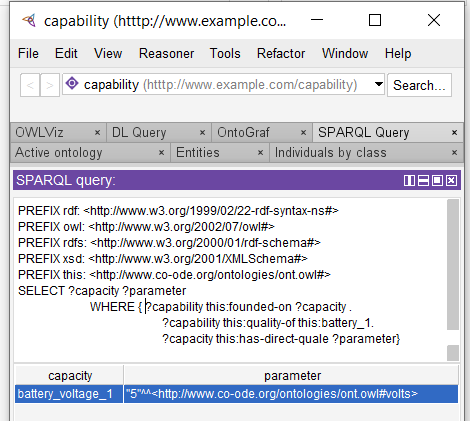
\includegraphics[width=0.45\textwidth]{query_screenshot.PNG}
  \caption{\label{fig:screen_query}}
\end{figure}

\begin{figure}
  \centering
  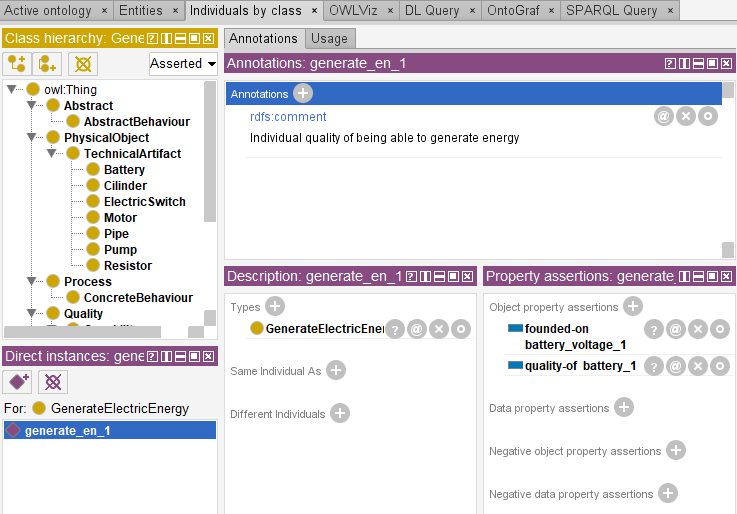
\includegraphics[width=0.45\textwidth]{entities_screenshot.PNG}
  \caption{\label{fig:screen_entities}}
\end{figure}

\section{Conclusion}\label{sec:conc}
\TODO{Riassumere cio' che e' stato detto nell'articolo. Ribadirne utilita'}



%\begin{figure}[t]
%\includegraphics{}
%\caption{Figure caption.}\label{f1}
%\end{figure}

%\begin{table*}
%\caption{} \label{t1}
%\begin{tabular}{lll}
%\hline
%&&\\
%&&\\
%\hline
%\end{tabular}
%\end{table*}

\section*{Acknowledgemnts}

%%%% NOTA:
%Tutte le pubblicazioni scientifiche eventualmente prodotte dal/dalla 
%dottorando/a che usufruisce della borsa finanziata dalla presente 
%Convenzione e derivate dall'attività svolta nell'ambito del ciclo 
%di dottorato, oltre a indicare l’afferenza al Dottorato dell’Università,
%dovrà citare il sostegno all’attività di ricerca da parte del Finanziatore.

The scholarship of Francesco Compagno is funded
by the company Adige Spa.

%%%%%%%%%%% The bibliography starts:

%%%%%%%%%%%%%%%%%%%%%%%%%%%%%%%%%%%%%%%%%%%%%%%%%%%%%%%%%%%%%
%%                  The Bibliography                       %%
%%                                                         %%
%%  ios1.bst will be used to                               %%
%%  create a .BBL file for submission.                     %%
%%                                                         %%
%%                                                         %%
%%  Note that the displayed Bibliography will not          %%
%%  necessarily be rendered by Latex exactly as specified  %%
%%  in the online Instructions for Authors.                %%
%%                                                         %%
%%%%%%%%%%%%%%%%%%%%%%%%%%%%%%%%%%%%%%%%%%%%%%%%%%%%%%%%%%%%%


%\nocite{*}
% if your bibliography is in bibtex format, use those commands:
\bibliographystyle{ios1}           % Style BST file.
\bibliography{bibliography}        % Bibliography file (usually '*.bib')

% or include bibliography directly:
%\begin{thebibliography}{0}
%\bibitem{r1} F. Author, Information about cited object.
%
%\bibitem{r2} S. Author and T. Author, Information about cited object.
%\end{thebibliography}

\end{document}
